\chapter{State of the Art} \label{chap:sota}

\section*{}
%Neste capítulo é descrito o estado da arte e são apresentados trabalhos relacionados para mostrar o que existe no mesmo domínio e quais os problemas em aberto. Deve deixar claro que existe uma oportunidade de desenvolvimento que cobre alguma falha concreta .

%O capítulo deve também efetuar uma revisão tecnológica às principais ferramentas utilizáveis no âmbito do projeto, justificando futuras escolhas.


The topic of blockchain oracles is still unexplored territory mostly investigated by start-up companies and individuals thriving to solve a new problem. Therefore, research related to oracles may not yet be documented on peer-reviewed papers but, nonetheless, is invaluable in an early phase of the technology. Consequently, the state of the art cannot be complete without reviewing the work developed by the academia and also by start-ups, enterprises, governments and individuals.

\section{Research}

To get an overview of academic research a systematic literature review was performed. It's main components and finding are described in this section.

A literature review allows scholars not to step on each other's shoes but to climb on each other's shoulders \cite{Kitchenham2007GuidelinesEngineering}, meaning, not duplicating existing research and find the gaps and strive to discover something new. To conduct a non-biased, methodical and reproducible review, to the extent that a human can, it is necessary to clarify and identify at the beginning of the research its methodology, what are the data sources and what is the selection criteria.

\subsection{Research Questions}
First of all and to guide the focus of the research, the following research question was defined:
\begin{itemize}
  \item RQ1: What kind of blockchain oracles have been proposed?
  \item RQ2: What are the research trends on blockchain oracles?
\end{itemize}


\subsection{Search Strategy and Data-sources}
Figure \ref{fig:/figures/SLR_stages}, presents the predefined review strategy used in order to achieve such a goal and maintain unbiased, transparent and reproducible research.

\begin{figure*}[t]
  \begin{center}
    \leavevmode
    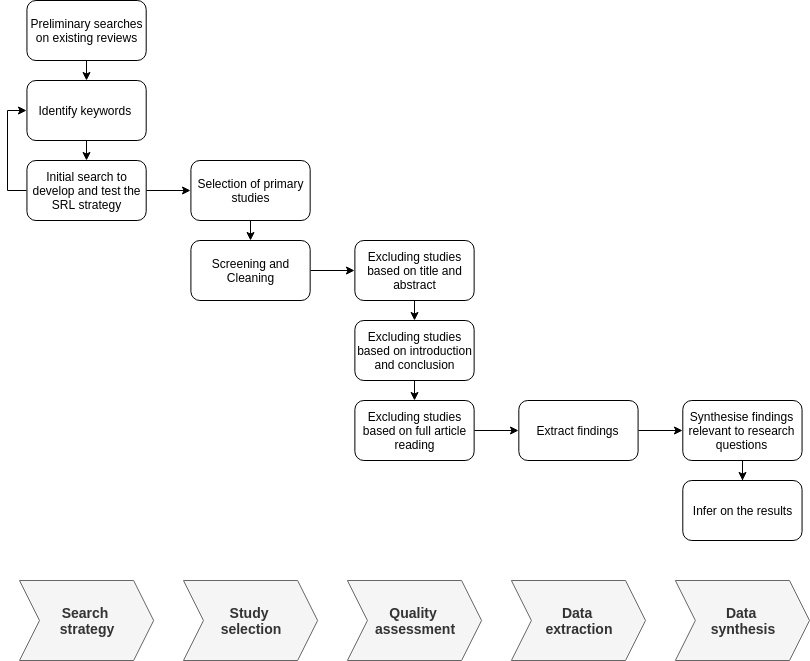
\includegraphics[width=\textwidth]{SLR_stages.png}
    \caption{Review strategy.}
    \label{fig:/figures/SLR_stages}
  \end{center}
\end{figure*}

The following four electronic databases were used to query for such information:

\begin{itemize}
  \item ACM Digital Library
  \item IEEE Xplore
  \item Scopus
  \item Google Scholar
\end{itemize}


The defined search query for the search of the relevant papers was the following:

(("blockchain" OR "block chain" OR "block-chain")
AND
("oracles" OR "oracle" OR "middle-ware" OR "middleware" OR "middle ware" OR "datafeed" OR "data feed" OR "data-feed"))

This search query was used to comprise all the possible ways of referring to blockchain and oracles. Some scholars have investigated the oracle issue by simply calling them a middleware or data-feed since oracles can either be used as an intermediary that relays data or as the source of the data.

The search was performed on the 5th of February 2019 and revealed the results presented in Table \ref{search-results-table}.

\begin{table}[H]
  \centering
  \begin{tabular}{llr}
    \hline
    \textbf{Database}   & \textbf{Filters}                & \textbf{Results} \\ \hline
    ACM Digital Library & Title, abstract and keywords    & 34               \\
    IEEE Xplore         & Title, abstract and index terms & 24               \\
    Scopus              & Title, abstract and keywords    & 57               \\
    Google Scholar      & Title                           & 8                \\ \hline
    \textbf{Total}      & \textbf{}                       & \textbf{123}     \\ \hline
  \end{tabular}
  \caption{Number of results and applied filters per database}
  \label{search-results-table}
\end{table}

Since the concept of smart contracts on the blockchain was only introduced in 2015, with the introduction of the Ethereum blockchain, only results after 2015 were considered, also, all duplicated papers were removed. Analysing the initial search results per year, in Figure \ref{search-results-per-year}, we can infer the growing popularity of oracle-related academic research. The year 2019 only comprises work done in the month of January since the search was performed at the beginning of February.

\begin{figure}[H]
  \centering
  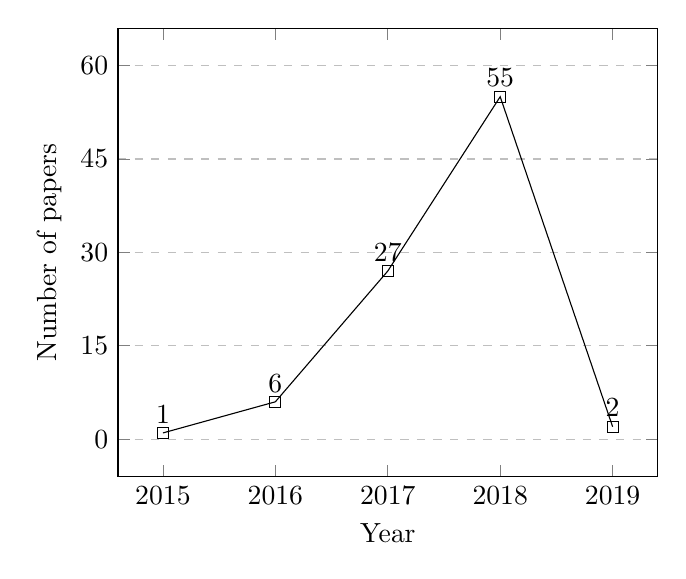
\begin{tikzpicture}
    \begin{axis}[
        xlabel={Year},
        ylabel={Number of papers},
        xtick=data,
        x tick label style={
            /pgf/number format/1000 sep=},
        xmin=2015, xmax=2019,
        ymin=0, ymax=60,
        ytick={0,15,30,45,60,75},
        ymajorgrids=true,
        grid style=dashed,
        enlargelimits=0.10,
      ]

      \addplot[
        mark=square, nodes near coords
      ]
      coordinates {
          (2015,1)(2016,6)(2017,27)(2018,55)(2019,2)
        };

    \end{axis}
  \end{tikzpicture}
  \caption{Resulting papers from search distributed per year}
  \label{search-results-per-year}
\end{figure}


\subsection{Study Selection and Quality Assessment}

The study selection process initially started with a pool of 123 papers from the previously stated online databases. As described on Figure \ref{fig:/figures/SLR_stages}, the selection compromised four stages:
\begin{itemize}
  \item Stage 1: Screening and cleaning duplicated articles or articles that were not in English.
  \item Stage 2: Exclusion by carefully reading the title but most importantly the abstract. After this stage, only 13 of the 91 non-duplicated papers were either describing specific trustable oracle implementations or mentioning the use of oracles.
  \item Stage 3: Analysing the introduction and conclusions in order to remove papers which do not describe an implementation of a trustable oracle or a protocol to overcome the trust in oracles.
  \item Stage 4: Full article reading to assess if the final bucket of articles answers the research questions.
\end{itemize}

The process of exclusion is depicted in Figure \ref{fig:/figures/paper-screening} and all the information regarding the papers and in which phase they were excluded is transparently presented in Appendix \ref{ap1:slr}.

\begin{figure*}[t]
  \begin{center}
    \leavevmode
    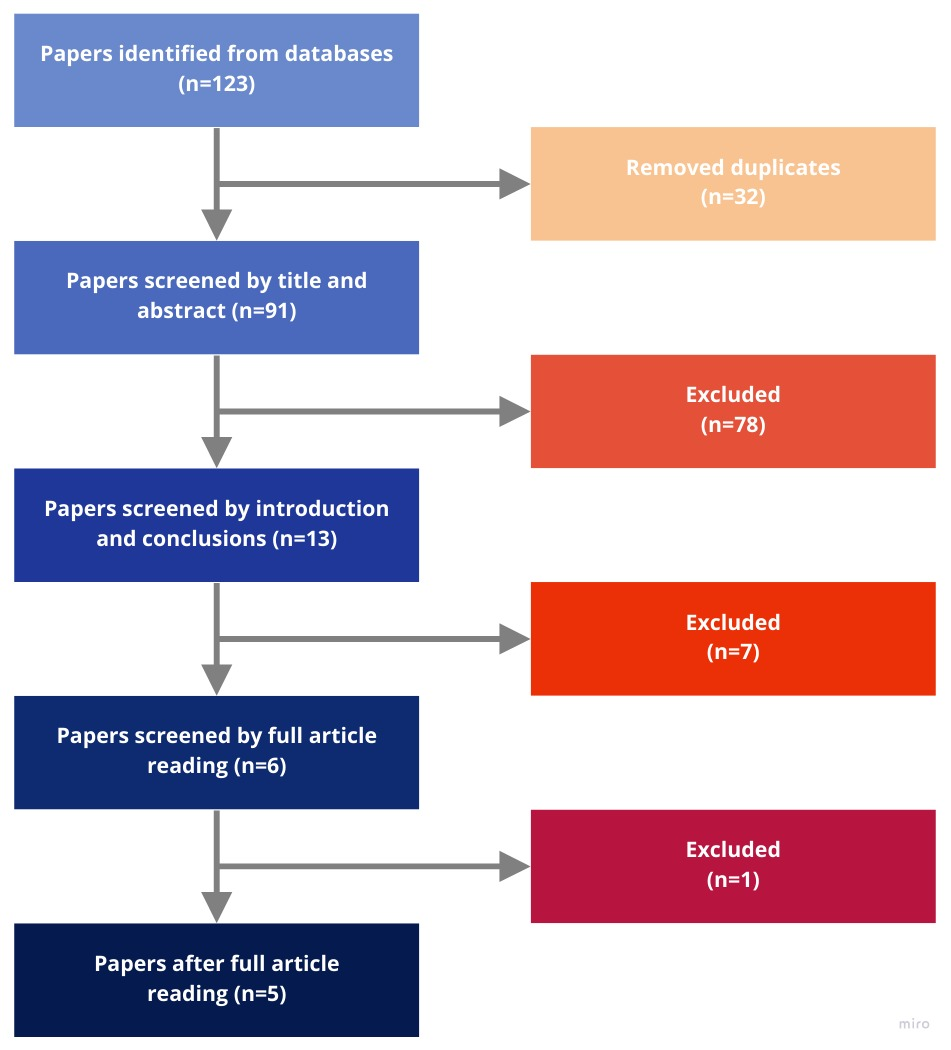
\includegraphics[width=0.7\textwidth]{figures/paper-screening.jpg}
    \caption{Screening stages.}
    \label{fig:/figures/paper-screening}
  \end{center}
\end{figure*}

\subsection{Data extraction and Data Synthesis}

The following process resulted in three articles and two theses that approach varying problems in implementing and guaranteeing trust in oracles.

Town Crier \cite{Zhang2016TownCrier}, leverages trusted hardware, specifically Intel SGX, to scrape HTTPS-enabled websites and serve source-authenticated data to relaying smart contracts. TC architecture involves a TC contract on the blockchain that receives datagram requests from a User Contract on the blockchain and communicates those request to a TC server which then retrieves an answer from a data source through an HTTPS connection.

Astraea \cite{Adler2018Astraea:Oracleb} proposes a decentralized oracle network with submitters, voters and certifiers, in which voters play a low-risk game and certifies a high-risk game with associated resources. Using game theory incentive structure as a means to keep the players honest.

Gilroy Gordon \cite{Gordon2017ProvenanceSensorsb} proposes a protocol for oracle sensor data authenticity and integrity to an IoT devices network with low computational resources. Using sets of public and private keys to authenticate that the oracle sensor data actually was originated by that oracle even if the information needs to pass by several oracles before being consumed by the application.

Francisco Monroy \cite{MontotoMonroy2018BitcoinBlockchain} defines a gambling protocol based on incentives and assuming that every entity involved has the objective to maximize their profit. The protocol overcomes the trust in a single Oracle by polling a network of 7 oracles from a large network of available oracles, they will then stake their money on a specific bet and only receive their investment back if the majority of the oracles vote in the same winner. Creating, therefore, incentives for Oracle good behaviour.

J. Eberhardt \cite{Eberhardt2018Off-chainingComputations} does not propose a specific method but analyses existing solutions and define a systematic classification for existing trustable off-chain computation oracles. The authors identify the following off-chain computation oracles approaches:



\begin{itemize}
  \item \textit{Verifiable off-chain Computation}, a technique where a prover executes a computation and then publishes the result including a cryptographic proof attesting the computation’s correctness to the blockchain. An on-chain verifier then verifies the proof and persists the result in case of success. Identified existing solutions are zkSNARKs, Bulletproofs and zkSTARKs. zkSNARKs require a setup phase which is more expensive than naive execution. After the setup, however, proof size and verification complexity are extremely small and independent of circuit complexity. This amortization makes zkSNARKs especially efficient for computations executed repeatedly, which is usually the case for off-chain state transitions. While zkSTARKs and Bulletproofs require no setup, proof size and verification complexity grow with circuit complexity, which limits applicability.
  \item \textit{Secure Multiparty Computation}, SMPCs, enable a set of nodes to compute functions on secret data in a way that none of the nodes ever has access to the data in its entirety. Identifies Enigma, which proposes a privacy-preserving decentralized computation platform based on sMPCs where a blockchain stores a publicly verifiable audit trail. However, current sMPC protocols add too much overhead for such a network to be practical. Hence, Enigma now relies on Trusted Execution Environments
  \item \textit{Enclave-based Computation}, relying on Trusted Execution Environments (TEE) to execute computations off-chain. Identified existing solutions are Enigma and Ekiden which present two different implementations of EOCs. In Enigma, programs can either be executed on-chain or in enclaves that are distributed across a separate off-chain network. An Enigma-specific scripting language allows developers to mark objects as private and hence, enforce off-chain computation. In contrast to Enigma, Ekiden does not allow on-chain computation but instead, the blockchain is solely used as persistent state storage.
  \item \textit{Incentive-driven Off-chain Computation}, IOC, relies on incentive mechanisms applied to motivate off-chain computation and guarantee computational correctness. IOCs inherit two critical design issues: (1) Keep verifiers motivated to validate solutions and (2) reduce computational effort for the on-chain judge. The paper identifies TrueBit, as the first IOC implementation, proposing solutions for both challenges. As verifiers would stop validating if solvers only published correct solutions, TrueBit enforces solvers to provide erroneous solutions from time to time and offers a reward to the verifiers for finding them.
\end{itemize}



\section{Non-Academia Research}

To search for non-academic research Google, a search engine and Medium, a platform for blog posting used widely by developers and the start-up community, were used as a means to find new projects or solutions for the oracle trust problem. Using these two tools a lot of projects were found trying to solve the oracle trust problem and are solely documented on white-papers or on the companies website documentation page. This kind of literature cannot be found in peer-reviewed databases, but can nonetheless provide invaluable information and is therefore worth being analysed.

The results of this search revealed a wide range of projects and protocols trying to achieve with varying degrees of decentralization or authenticity, a short explanation of each will be detailed here:

\begin{itemize}
  \item Oraclize.it \cite{Oraclize.it2018OraclizeDocumentation}, provides Authenticity Proofs for the data it fetches guaranteeing that the original data-source is genuine and untampered and can even make use of several data sources in order the gather trustable data, but its centralized model does not guarantee an always available service.
  \item ChainLink\cite{Ellis2017ChainLinkNetwork}, describes a decentralized network of oracles that can query multiple sources in order to avoid dependency of a sole oracle which can be prone to fail and also to gather knowledge from multiple sources to obtain a more reliable result. ChainLink is also considering implementing, in the future, authenticity proofs and make use of trusted hardware, as of now it requires users to trust in the ChainLink nodes to behave correctly.
  \item SchellingCoin protocol incentivizes a decentralized network of oracles
        to perform computation by rewarding participants who submit results
        that are closest to the median of all submitted results in a commit-reveal
        process.
  \item TrueBit, introduces a system of solvers and verifier. Solvers are
        compensated for performing computation and verifiers are compensated
        for detecting errors in solutions submitted by solvers.
\end{itemize}


\section{Summary and Conclusions}

Summing up, this research highlighted two main types of oracles. The first is \textbf{Data-Carrier oracles}, whose main purpose is relaying query results from a trusted data source to a smart contract. The second is \textbf{Computation Oracles}, which not only relay query results but also perform the relevant computation themselves. Computation oracles can be used as building blocks to construct off-chain computation markets. A summary of the results is described in Table \ref{oracle-summary}.

\begin{table}[]
  \centering
  \begin{tabular}{llll}
    \hline
    Name                                      & Type         & Distributed Network & Achieves trust through               \\ \hline
    Town Crier                                & Data carrier & No                  & Trusted hardware signed attestations \\
    Astraea                                   & Data carrier & Yes                 & Game theory incentives               \\
    \cite{Gordon2017ProvenanceSensorsb}       & Computation  & Yes                 & Sets of public and private keys      \\
    \cite{MontotoMonroy2018BitcoinBlockchain} & Data carrier & Yes                 & Incentive based                      \\
    TrueBit                                   & Computation  & Yes                 & Incentive based                      \\
    Oraclize.it                               & Data carrier & No                  & TLSNotary                            \\
    ChainLink                                 & Data carrier & Yes                 & Query multiple sources               \\
    SchellingCoin                             & Computation  & Yes                 & Incentive based                      \\ \hline
  \end{tabular}
  \caption{Summary of oracle projects/research.}
  \label{oracle-summary}
\end{table}

Two main conclusions come from both academic and non-academic research.

First of all, there is a clear lack of academic research on the topic of creating trustable oracles. Town Crier proposes a solution for relaying data securely but requiring specific hardware. Astraea and \cite{MontotoMonroy2018BitcoinBlockchain} uses incentives and game theory as a means for good oracle behaviour but does not provide complete trust in edge cases in which pursing erratic behaviour may be worth it.

\cite{Eberhardt2018Off-chainingComputations} is very promising in the field of Internet of Things for oracle sensor authentication but can only guarantee that data was generated by a specific sensor but the approach cannot be generalised for other oracle scenarios.

Secondly, even though the main research on trustable oracles is being pursued by startups or sole developers all the existing projects seem to be blockchain specific or in very early phases and not yet ready to be generally adopted.

The literature review points out the lack of research done by the academic in trying to solve one of the most important motives for blockchain general adoption. Only second, maybe, to scalability. The oracle trust problem, efficiently solved, opens doors to the contracts of the futures. Start-ups and sole developers are for now the main force in solving this problem which launches the challenge and motivation for the next chapter of this research.